\documentclass[a4paper,12pt]{article}

\usepackage{latexsym}
\usepackage[utf8]{inputenc}
\usepackage{graphicx}
\usepackage{amsmath}
\usepackage{float}% If comment this, figure moves to Page 2
\usepackage{longtable}

\author{Krzysztof~Palka and Dominik~Odrowski}
\date{April 4, 2013}

\title{\textsc{Exercise} 417 \\ Diffraction and interfere interference of light.} 

\addtolength{\textwidth}{2.5cm}
\addtolength{\hoffset}{-1.25cm}

\begin{document}

\maketitle

\begin{abstract}
This report presents examination of diffraction and interference of light on diffraction grading and, basing on those phenomenas determination of sizes of slits.  
\end{abstract}

\section{Introduction}
The aim of this exercise was to determine size of slits in diffraction grading using experimental set-up based on He-Ne laser.

\section{Theory and measurement}
When beam of laser light encounters diffraction grading, then in result of diffraction every slit becomes a source of new wave (Huygens wavelets). Because of interference phenomena intensity of waves could grow or fall. When we cope with many slits, we can see on the screen many fringes in places, where occurs interference maximum. We can measure intensity if interfered waves using phototransistor. To make task easier we can put phototransistor in one place and displace fringes, when we know value of this displacement. 

\begin{figure}[H]
\begin{center}
    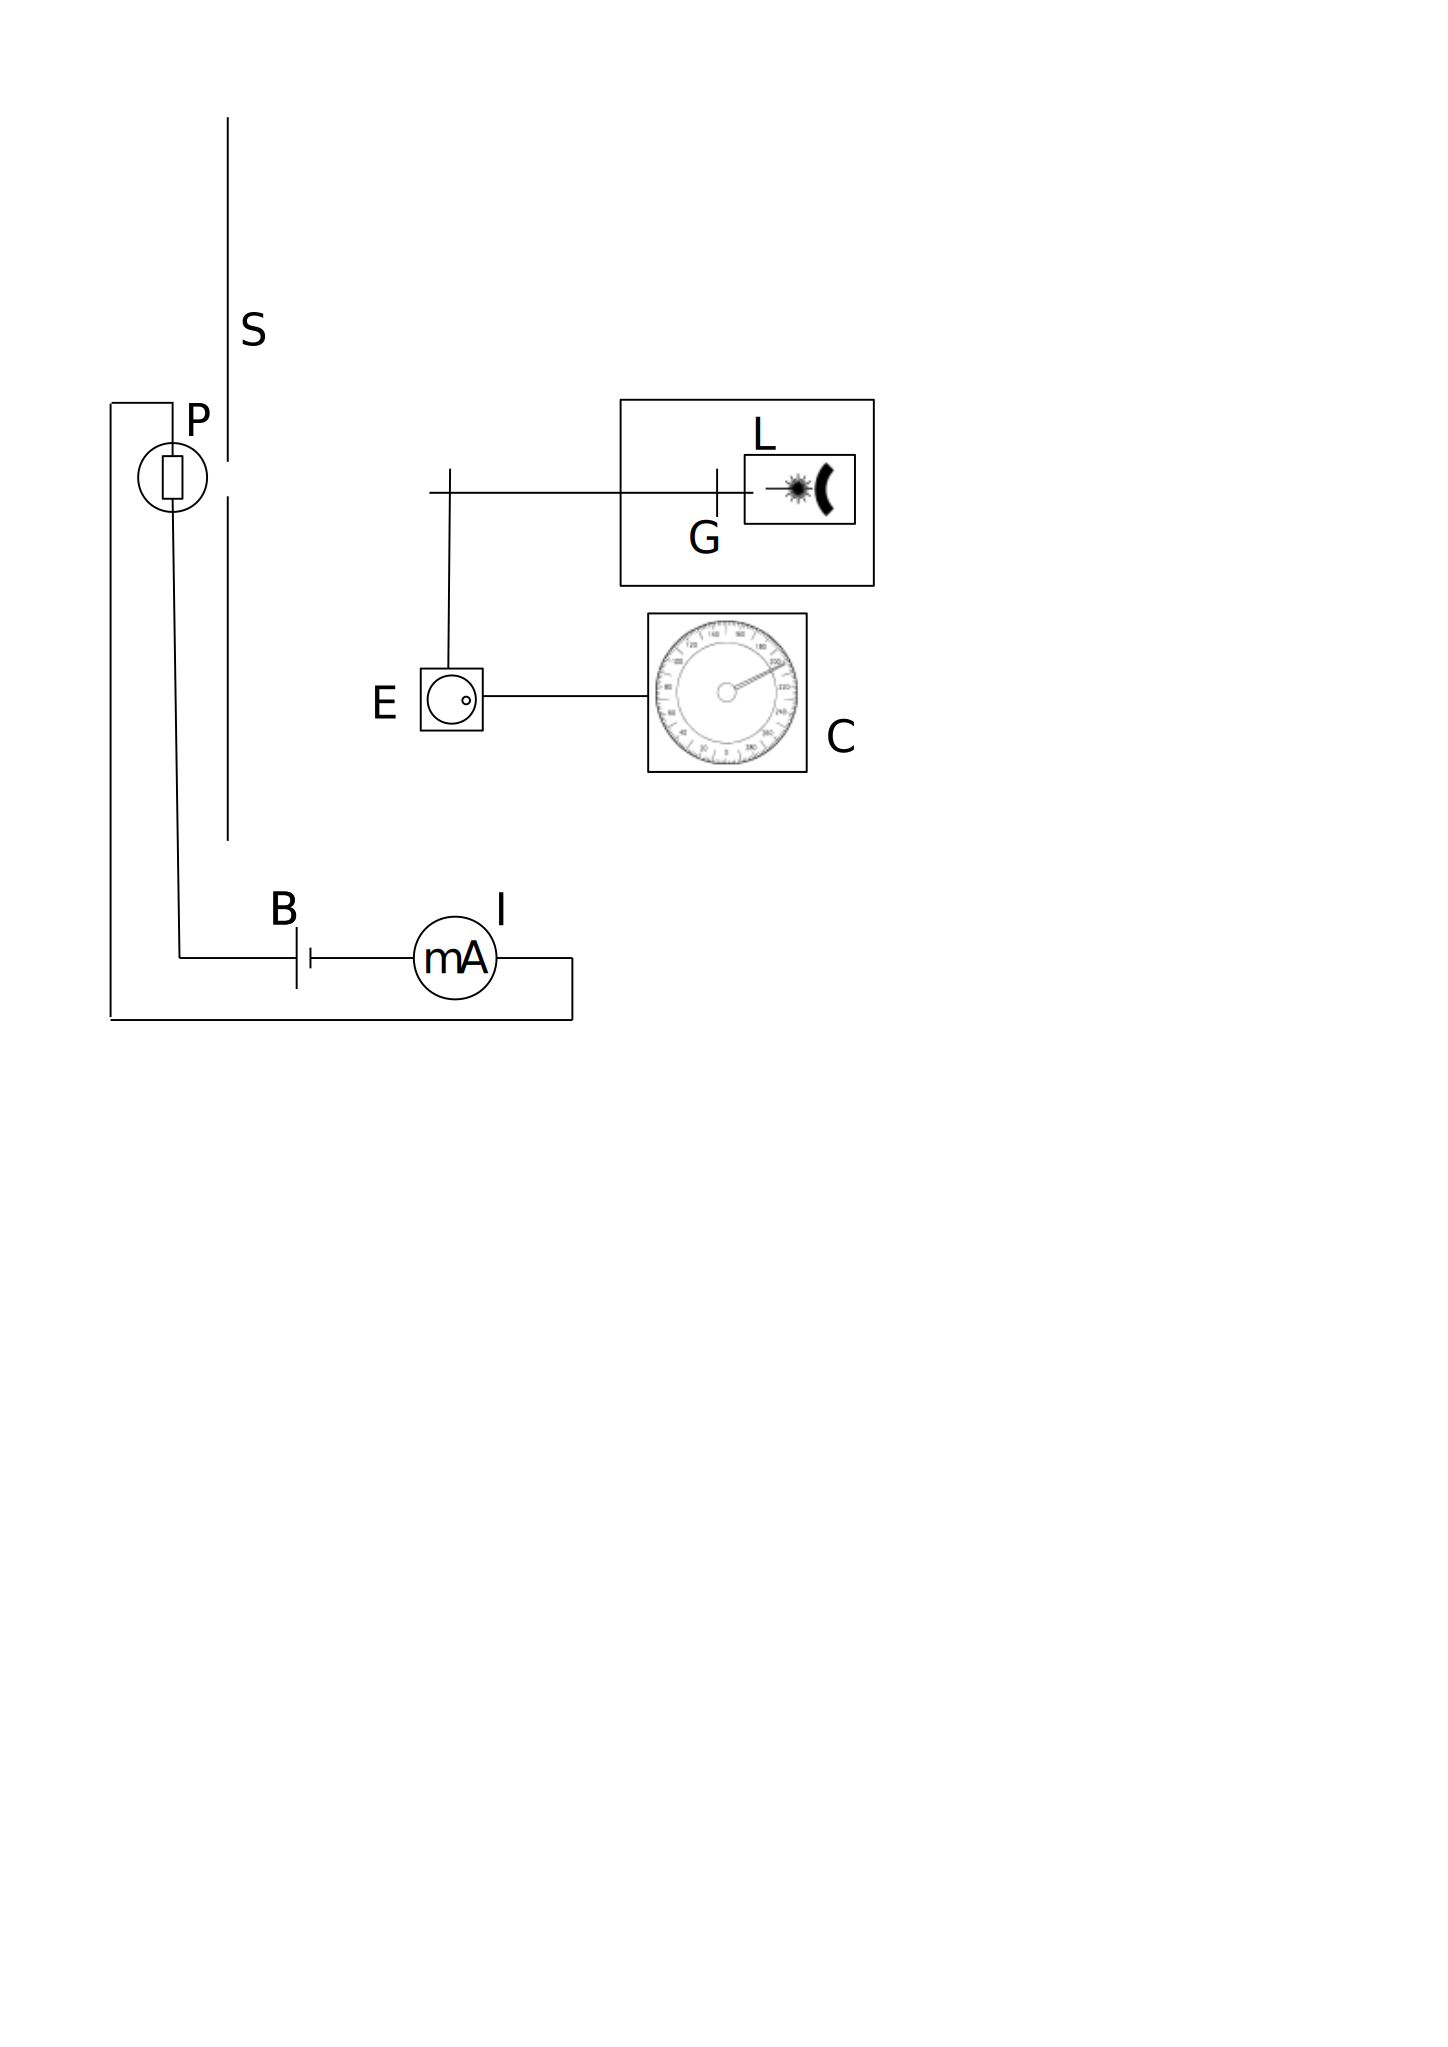
\includegraphics[width=0.6\textwidth]{set-up}
    \caption{Diagram of experimental set-up. It consists of a He-Ne laser (L), diffraction grading (G), laser and diffraction grading displacement setter (E), impulse counter (C), screen (S), phototransistor (P), 9V battery (B) and microamperometer (I).}
    \label{fig:set-up}
\end{center}
\end{figure}

\section{Results}
We can measure intensity of particular fringes by moving laser and diffraction grading using arm. Angle of displacement can by measured thanks to impulse counter (impulses are send by setter). One impulse means displacement of the image by 0.2 mrad. 

\begin{center}
\begin{longtable}{|c|c|c||c|c|c|}
\caption[Feasible triples for a highly variable Grid]
{Results of measurements, uncertainty for DMM Escort-95T (0.2\%+30d) } \label{grid_mlmmh} \\

\hline 
\multicolumn{1}{|c|}{\textbf{Impulses}} & 
\multicolumn{1}{|c|}{\textbf{Angle [mrad]}} & 
\multicolumn{1}{|c||}{\textbf{Current [I]}} & 
\multicolumn{1}{|c|}{\textbf{Impulses}} & 
\multicolumn{1}{|c|}{\textbf{Angle [mrad]}} & 
\multicolumn{1}{|c|}{\textbf{Current [I]}} \\ \hline 
\endfirsthead

\multicolumn{6}{c}%
{{\bfseries \tablename\ \thetable{} -- continued from previous page}} \\
\hline 
\multicolumn{1}{|c|}{\textbf{Impulses}} &
\multicolumn{1}{c|}{\textbf{Angle [mrad]}} &
\multicolumn{1}{c||}{\textbf{Current [I]}} & 
\multicolumn{1}{|c|}{\textbf{Impulses}} &
\multicolumn{1}{c|}{\textbf{Angle [mrad]}} &
\multicolumn{1}{c|}{\textbf{Current [I]}} \\ \hline 
\endhead

\hline \multicolumn{6}{|r|}{{Continued on next page}} \\ \hline
\endfoot

\hline \hline
\endlastfoot

0 & -22.8 & 28.2 $\pm$  3.1   & 540 & -1.2 & 1788 $\pm$  34  \\
5 & -22.6 & 30.4 $\pm$  3.1   & 545 & -1.0 & 1752 $\pm$  34  \\
10 & -22.4 & 29.2 $\pm$  3.1   & 550 & -0.8 & 1755 $\pm$  34  \\
15 & -22.2 & 29.8 $\pm$  3.1   & 555 & -0.6 & 2359 $\pm$  35  \\
20 & -22.0 & 32.4 $\pm$  3.1   & 560 & -0.4 & 3058 $\pm$  36  \\
25 & -21.8 & 31.1 $\pm$  3.1   & 565 & -0.2 & 3407 $\pm$  37  \\
30 & -21.6 & 35.4 $\pm$  3.1   & 570 & 0.0 & 3728 $\pm$  37  \\
35 & -21.4 & 37.5 $\pm$  3.1   & 575 & 0.2 & 3648 $\pm$  37  \\
40 & -21.2 & 38.6 $\pm$  3.1   & 580 & 0.4 & 3452 $\pm$  37  \\
45 & -21.0 & 42.0 $\pm$  3.1   & 585 & 0.6 & 2988 $\pm$  36  \\
50 & -20.8 & 42.0 $\pm$  3.1   & 590 & 0.8 & 1303 $\pm$  33  \\
55 & -20.6 & 39.8 $\pm$  3.1   & 595 & 1.0 & 612 $\pm$  31  \\
60 & -20.4 & 38.0 $\pm$  3.1   & 600 & 1.2 & 2812 $\pm$  36  \\
65 & -20.2 & 38.8 $\pm$  3.1   & 605 & 1.4 & 1272 $\pm$  33  \\
70 & -20.0 & 38.5 $\pm$  3.1   & 610 & 1.6 & 1039 $\pm$  32  \\
75 & -19.8 & 38.3 $\pm$  3.1   & 615 & 1.8 & 1066 $\pm$  32  \\
80 & -19.6 & 37.4 $\pm$  3.1   & 620 & 2.0 & 1023 $\pm$  32  \\
85 & -19.4 & 33.8 $\pm$  3.1   & 625 & 2.2 & 1147 $\pm$  32  \\
90 & -19.2 & 18.6 $\pm$  3.0   & 630 & 2.4 & 1341 $\pm$  33  \\
95 & -19.0 & 14.8 $\pm$  3.0   & 635 & 2.6 & 1336 $\pm$  33  \\
100 & -18.8 & 11.8 $\pm$  3.0   & 640 & 2.8 & 1330 $\pm$  33  \\
105 & -18.6 & 10.8 $\pm$  3.0   & 645 & 3.0 & 1215 $\pm$  32  \\
110 & -18.4 & 9.7 $\pm$  3.0   & 650 & 3.2 & 1171 $\pm$  32  \\
115 & -18.2 & 8.7 $\pm$  3.0   & 655 & 3.4 & 1054 $\pm$  32  \\
120 & -18.0 & 4.9 $\pm$  3.0   & 660 & 3.6 & 1069 $\pm$  32  \\
125 & -17.8 & 4.0 $\pm$  3.0   & 665 & 3.8 & 1077 $\pm$  32  \\
130 & -17.6 & 2.8 $\pm$  3.0   & 670 & 4.0 & 1024 $\pm$  32  \\
135 & -17.4 & 2.1 $\pm$  3.0   & 675 & 4.2 & 565 $\pm$  31  \\
140 & -17.2 & 1.3 $\pm$  3.0   & 680 & 4.4 & 512 $\pm$  31  \\
145 & -17.0 & 1.1 $\pm$  3.0   & 685 & 4.6 & 478 $\pm$  31  \\
150 & -16.8 & 1.2 $\pm$  3.0   & 690 & 4.8 & 448 $\pm$  31  \\
155 & -16.6 & 1.2 $\pm$  3.0   & 695 & 5.0 & 442 $\pm$  31  \\
160 & -16.4 & 1.2 $\pm$  3.0   & 700 & 5.2 & 506 $\pm$  31  \\
165 & -16.2 & 1.2 $\pm$  3.0   & 705 & 5.4 & 343.2 $\pm$  3.7  \\
170 & -16.0 & 1.2 $\pm$  3.0   & 710 & 5.6 & 281.2 $\pm$  3.6  \\
175 & -15.8 & 1.4 $\pm$  3.0   & 715 & 5.8 & 262.4 $\pm$  3.5  \\
180 & -15.6 & 2.9 $\pm$  3.0   & 720 & 6.0 & 182.2 $\pm$  3.4  \\
185 & -15.4 & 13.0 $\pm$  3.0   & 725 & 6.2 & 137.8 $\pm$  3.3  \\
190 & -15.2 & 17.9 $\pm$  3.0   & 730 & 6.4 & 104.6 $\pm$  3.2  \\
195 & -15.0 & 27.3 $\pm$  3.1   & 735 & 6.6 & 83.7 $\pm$  3.2  \\
200 & -14.8 & 35.4 $\pm$  3.1   & 740 & 6.8 & 52.3 $\pm$  3.1  \\
205 & -14.6 & 33.9 $\pm$  3.1   & 745 & 7.0 & 39.3 $\pm$  3.1  \\
210 & -14.4 & 36.5 $\pm$  3.1   & 750 & 7.2 & 30.1 $\pm$  3.1  \\
215 & -14.2 & 52.2 $\pm$  3.1   & 755 & 7.4 & 25.1 $\pm$  3.1  \\
220 & -14.0 & 56.1 $\pm$  3.1   & 760 & 7.6 & 17.6 $\pm$  3.0  \\
225 & -13.8 & 62.8 $\pm$  3.1   & 765 & 7.8 & 12.0 $\pm$  3.0  \\
230 & -13.6 & 62.3 $\pm$  3.1   & 770 & 8.0 & 9.1 $\pm$  3.0  \\
235 & -13.4 & 62.7 $\pm$  3.1   & 775 & 8.2 & 6.6 $\pm$  3.0  \\
240 & -13.2 & 91.1 $\pm$  3.2   & 780 & 8.4 & 4.2 $\pm$  3.0  \\
245 & -13.0 & 100.5 $\pm$  3.2   & 785 & 8.6 & 2.9 $\pm$  3.0  \\
250 & -12.8 & 107.4 $\pm$  3.2   & 790 & 8.8 & 2.3 $\pm$  3.0  \\
255 & -12.6 & 118.2 $\pm$  3.2   & 795 & 9.0 & 2.3 $\pm$  3.0  \\
260 & -12.4 & 128.3 $\pm$  3.3   & 800 & 9.2 & 2.5 $\pm$  3.0  \\
265 & -12.2 & 130.1 $\pm$  3.3   & 805 & 9.4 & 2.5 $\pm$  3.0  \\
270 & -12.0 & 125.2 $\pm$  3.3   & 810 & 9.6 & 2.6 $\pm$  3.0  \\
275 & -11.8 & 132.2 $\pm$  3.3   & 815 & 9.8 & 6.2 $\pm$  3.0  \\
280 & -11.6 & 132.7 $\pm$  3.3   & 820 & 10.0 & 8.1 $\pm$  3.0  \\
285 & -11.4 & 127.7 $\pm$  3.3   & 825 & 10.2 & 10.2 $\pm$  3.0  \\
290 & -11.2 & 123.3 $\pm$  3.2   & 830 & 10.4 & 12.4 $\pm$  3.0  \\
295 & -11.0 & 116.3 $\pm$  3.2   & 835 & 10.6 & 8.0 $\pm$  3.0  \\
300 & -10.8 & 111.9 $\pm$  3.2   & 840 & 10.8 & 9.4 $\pm$  3.0  \\
305 & -10.6 & 107.6 $\pm$  3.2   & 845 & 11.0 & 11.5 $\pm$  3.0  \\
310 & -10.4 & 109.7 $\pm$  3.2   & 850 & 11.2 & 15.4 $\pm$  3.0  \\
315 & -10.2 & 109.7 $\pm$  3.2   & 855 & 11.4 & 22.4 $\pm$  3.0  \\
320 & -10.0 & 107.5 $\pm$  3.2   & 860 & 11.6 & 22.1 $\pm$  3.0  \\
325 & -9.8 & 67.5 $\pm$  3.1   & 865 & 11.8 & 21.5 $\pm$  3.0  \\
330 & -9.6 & 49.2 $\pm$  3.1   & 870 & 12.0 & 22.8 $\pm$  3.0  \\
335 & -9.4 & 34.9 $\pm$  3.1   & 875 & 12.2 & 22.3 $\pm$  3.0  \\
340 & -9.2 & 20.9 $\pm$  3.0   & 880 & 12.4 & 19.4 $\pm$  3.0  \\
345 & -9.0 & 13.2 $\pm$  3.0   & 885 & 12.6 & 17.8 $\pm$  3.0  \\
350 & -8.8 & 9.9 $\pm$  3.0   & 890 & 12.8 & 16.7 $\pm$  3.0  \\
355 & -8.6 & 10.7 $\pm$  3.0   & 895 & 13.0 & 16.8 $\pm$  3.0  \\
360 & -8.4 & 6.5 $\pm$  3.0   & 900 & 13.2 & 16.1 $\pm$  3.0  \\
365 & -8.2 & 6.5 $\pm$  3.0   & 905 & 13.4 & 15.7 $\pm$  3.0  \\
370 & -8.0 & 8.5 $\pm$  3.0   & 910 & 13.6 & 15.1 $\pm$  3.0  \\
375 & -7.8 & 14.2 $\pm$  3.0   & 915 & 13.8 & 14.8 $\pm$  3.0  \\
380 & -7.6 & 23.4 $\pm$  3.0   & 920 & 14.0 & 15.0 $\pm$  3.0  \\
385 & -7.4 & 41.2 $\pm$  3.1   & 925 & 14.2 & 6.9 $\pm$  3.0  \\
390 & -7.2 & 82.1 $\pm$  3.2   & 930 & 14.4 & 5.0 $\pm$  3.0  \\
395 & -7.0 & 147.6 $\pm$  3.3   & 935 & 14.6 & 5.0 $\pm$  3.0  \\
400 & -6.8 & 215.3 $\pm$  3.4   & 940 & 14.8 & 4.0 $\pm$  3.0  \\
405 & -6.6 & 287.1 $\pm$  3.6   & 945 & 15.0 & 4.7 $\pm$  3.0  \\
410 & -6.4 & 392.0 $\pm$  3.8   & 950 & 15.2 & 7.2 $\pm$  3.0  \\
415 & -6.2 & 423 $\pm$  31   & 955 & 15.4 & 5.9 $\pm$  3.0  \\
420 & -6.0 & 400 $\pm$  31   & 960 & 15.6 & 2.3 $\pm$  3.0  \\
425 & -5.8 & 642 $\pm$  31   & 965 & 15.8 & 2.0 $\pm$  3.0  \\
430 & -5.6 & 980 $\pm$  32   & 970 & 16.0 & 1.7 $\pm$  3.0  \\
435 & -5.4 & 1079 $\pm$  32   & 975 & 16.2 & 1.4 $\pm$  3.0  \\
440 & -5.2 & 1106 $\pm$  32   & 980 & 16.4 & 1.0 $\pm$  3.0  \\
445 & -5.0 & 1159 $\pm$  32   & 985 & 16.6 & 0.9 $\pm$  3.0  \\
450 & -4.8 & 1187 $\pm$  32   & 990 & 16.8 & 0.9 $\pm$  3.0  \\
455 & -4.6 & 1368 $\pm$  33   & 995 & 17.0 & 0.7 $\pm$  3.0  \\
460 & -4.4 & 1572 $\pm$  33   & 1000 & 17.2 & 0.8 $\pm$  3.0  \\
465 & -4.2 & 1880 $\pm$  34   & 1005 & 17.4 & 1.0 $\pm$  3.0  \\
470 & -4.0 & 2117 $\pm$  34   & 1010 & 17.6 & 1.2 $\pm$  3.0  \\
475 & -3.8 & 2404 $\pm$  35   & 1015 & 17.8 & 1.5 $\pm$  3.0  \\
480 & -3.6 & 2612 $\pm$  35   & 1020 & 18.0 & 0.8 $\pm$  3.0  \\
485 & -3.4 & 2633 $\pm$  35   & 1025 & 18.2 & 1.0 $\pm$  3.0  \\
490 & -3.2 & 2523 $\pm$  35   & 1030 & 18.4 & 1.5 $\pm$  3.0  \\
495 & -3.0 & 2521 $\pm$  35   & 1035 & 18.6 & 2.4 $\pm$  3.0  \\
500 & -2.8 & 2522 $\pm$  35   & 1040 & 18.8 & 2.5 $\pm$  3.0  \\
505 & -2.6 & 2268 $\pm$  35   & 1045 & 19.0 & 2.5 $\pm$  3.0  \\
510 & -2.4 & 2132 $\pm$  34   & 1050 & 19.2 & 2.7 $\pm$  3.0  \\
515 & -2.2 & 1906 $\pm$  34   & 1055 & 19.4 & 3.0 $\pm$  3.0  \\
520 & -2.0 & 1788 $\pm$  34   & 1060 & 19.6 & 2.5 $\pm$  3.0  \\
525 & -1.8 & 2023 $\pm$  34   & 1065 & 19.8 & 2.6 $\pm$  3.0  \\
530 & -1.6 & 2186 $\pm$  34   & 1070 & 20.0 & 2.7 $\pm$  3.0  \\
535 & -1.4 & 1805 $\pm$  34   & 1075 & 20.2 & 3.0 $\pm$  3.0  \\


\end{longtable}
\end{center}

To find interference maxima we will plot this data on graph. 

\begin{figure}[H]
    \begin{center}
        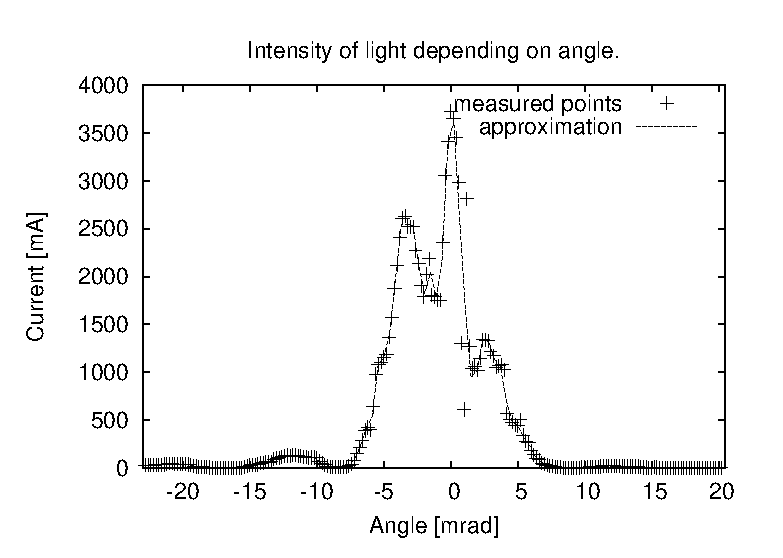
\includegraphics[width=0.90\textwidth]{plot}
        \caption{graph of measured current - indicator of intensity of light versus displaced angle}
        \label{fig:plot}
    \end{center}
\end{figure}

We would mark subsequent interference maxima - those with negative angle value (those with positive angle values seems to be less accurate) - as $m_1$, $m_2$, \dots. So, from the plot we can see that for $m_1$ angle is 1.6 mrad, for $m_2$ - 3.6 mrad and so on. It is enough to determine value of $d$. If we rewrite equation \ref{eq:imax1} for maxima - lines we would get eq. \ref{eq:imax2} from which we can calculate $d$.
\begin{equation}
    d \sin \theta = m \lambda \qquad \textrm{for $m$ = 1, 2, 3\dots (maxima - bright fringes)} \label{eq:imax1}
\end{equation}

\begin{equation}
    d = \frac{m \lambda}{\sin \theta} \label{eq:imax2}
\end{equation}

In analogous way we can find size of slits. For this purpose we would use equation \ref{eq:imin1}

\begin{equation}
    a \sin \theta = m \lambda \qquad \textrm{for $m$ = 1, 2, 3,\dots (minima - dark fringers)} \label{eq:imin1}
\end{equation}


Calculation of first 2 minima and maxima (that is all we managed to measured), calculation of average and standard derivation gives following results

\begin{displaymath}
    d = (4.6 \pm 0.9) \cdot 10^{-4} \, \mathrm{m}
\end{displaymath}

\begin{displaymath}
    a = (3.0 \pm 0.2) \cdot 10^{-4} \, \mathrm{m}
\end{displaymath}


And now, when we got approximate values of $a$ and $d$, we can put them to equation \ref{eq:IvsTheta} and get approximate plot of brightness of fringes made by used diffraction grading.

\section{Conclusions}
The most noticeable element of this report is plot of intensity of light. More precisely - its lack of symmetry. It could be caused by fast discharging of battery - during measurement of the lightest fringes there was quite high current in circuit, and decrement of read current has begun at that moment. The other reason could be need of change scale of multimeter (this moment can be noticed when we look on uncertainties in the table with results). But even in this situation local maxima and minima was symmetric according to axis that indicated angle. And if size of detector is consider - it can influent on results. When we look at plot of intensity we can notice, that there is smooth transition between values and bigger detector can catch some light not intended for particular angle.       


\begin{thebibliography}{9}
    \bibitem{HRW}\emph{Fundamentals of physics} (2011) [ebook]. David Halliday, Robert Resnick, Jearl Walker. 9th ed. ISBN 978-0-470-46908-8
\end{thebibliography}

\end{document}
